% Chapter 2
\chapter{Sécurité des réseaux}

\label{Chapter2} 

Les réseaux définis par logiciel sont une catégorie émergente de réseaux qui présente de nouveaux défis du point de vue sécurité. Ce chapitre fournit un aperçu complet sur les menaces de sécurité auxquelles est confrontée cette architecture émergente, en particulier les attaques par déni de service Dos. Différentes solutions déjà proposées pour sécuriser cette technologie vont être vues et examiner au cours de ce chapitre afin de mieux comprendre comment l'aspect de sécurité est géré au sein d'un réseau SDN, ce qui nous aidera par la suite à proposer une solution adéquate pour la détection des attaques DoS dans un tel réseau.

\section{Sécurité dans un réseau Informatique}

\subsection{Généralités}
La sécurité des réseaux informatiques est la stratégie et les dispositions d’une organisation pour assurer la sécurité de ses actifs et de tout le trafic réseau. Elle se manifeste par une mise en en œuvre des mécanismes qui sont conçues pour détecter, prévenir et lutter contre une attaque de sécurité et des services de sécurité qui augmentent la sécurité des traitements et des échanges de données d’un système. Un service de sécurité utilise un ou plusieurs mécanismes de sécurité.\\

\noindent Lors du développement d’un réseau sécurisé, il convient de prendre en compte les services suivants:\\
\begin{itemize}
\item[•]\textbf{L’authenticité}: L’identité des acteurs de la communication est vérifiée.\\
\item[•]\textbf{La confidentialité}: Les données (et l'objet et les acteurs) de la communication ne peuvent pas être connues d’un tiers non autorisé.\\
\item[•]\textbf{L’intégrité}: Les données de la communication n’ont pas été altérées.\\
\item[•]\textbf{La disponibilité}: Les acteurs de la communication accèdent aux données dans de bonnes conditions.\\
\item[•]\textbf{La non-répudiation}: Les acteurs impliqués dans la communication ne peuvent nier y avoir participé.
\end{itemize}

\newpage

\subsection{Les menaces d’un réseau informatique}
Une attaque est une action qui compromet la sécurité des informations. Les attaques peuvent être classées sous deux catégories:\\
\begin{itemize}
\item[\textbf{Attaque passive}]: consiste à écouter sans modifier les données ou le fonctionnement du réseau. Elles sont généralement indétectables mais une prévention est possible.\\
\item[\textbf{Attaque active}]: consiste à modifier des données ou des messages, à s'introduire dans des équipements réseau ou à perturber le bon fonctionnement de ce réseau. Noter qu'une attaque active peut être exécutée sans la capacité d'écoute.
\end{itemize}

\subsection{Les mécanismes de sécurité}
\begin{itemize}
\item[•]\textbf{Pare-feu}: un élément (logiciel ou matériel) du réseau informatique contrôlant les communications qui le traversent. Il a pour fonction de faire respecter la politique de sécurité du réseau, celle-ci définissant quels sont les communications autorisés ou interdits. N'empêche pas un attaquant d'utiliser une connexion autorisée pour attaquer le système. Ne protège pas contre une attaque venant du réseau intérieur (qui ne le traverse pas).\\
\item[•]\textbf{Antivirus}: logiciel sensé de protéger ordinateur contre les logiciels (ou fichiers potentiellement exécutables) néfastes. Ne protège pas contre un intrus qui emploie un logiciel légitime, ou contre un utilisateur légitime qui accède à une ressource alors qu'il n'est pas autorisé à le faire.\\
\item[•]\textbf{Détection d'intrusion}: repère les activités anormales ou suspectes sur le réseau surveillé. Ne détecte pas les accès incorrects mais autorisés par un utilisateur légitime. Mauvaise détection : taux de faux positifs, faux négatifs.\\
\item[•]\textbf{Contrôle d’accès}: vérifie les droits d’accès d'un acteur aux données. N'empêche pas l'exploitation d'une vulnérabilité.
\end{itemize}

\section{La sécurité dans les réseaux SDN}
le but des SDN est de rendre les réseaux traditionnels plus sécurisés et robustes. La gestion centralisée des SDN simplifie la façon dont les mécanismes de sécurité sont introduit dans le réseau. Cependant cette solution ouvre porte à d'autres types d'attaque. Attaque initiées à partir des applications de gestion malicieuses, attaques sur le contrôleur, compromettre les switches.\\\\
Selon Kreutz et al[\cite{7}], les vecteurs d'attaques identifiés dans les SDN sont décrits dans le tableau \ref{table:Threat_Vectors}.
\newpage
\begin{table}[h]
\begin{center}
\begin{tabular}{  m{0.5cm} m{11cm} }
\hline
\textbf{N}. & \textbf{Vecteur d'attaque}\\
\hline
1 & Flux de trafic falsifié ou truqué\\
2 & Attaques contre les vulnérabilités des commutateurs\\
3 & Attaque sur les liens de communication du contrôleur\\
4 & Attaques contre les vulnérabilités des contrôleurs\\
5 & Manque de mécanismes pour assurer la confiance entre le contrôleur
et application de gestion\\
6 & Attaques contre les vulnérabilités des postes administratifs\\
\hline
\end{tabular}
\caption{Vecteurs d'attaque}
\label{table:Threat_Vectors}
\end{center}
\end{table}

Parmi ces vecteurs d'attaques, numéro 3,4 et 5 ne sont pas présents dans les réseaux traditionnels. Ils sont spécifiques aux SDN. Ils résultent de la séparation du plan de contrôle et de données et de la centralisation logique des contrôleurs. D'autres vecteurs étaient déjà présentés dans les réseaux traditionnels.

\subsection{Les failles de sécurité des réseaux SDN}
Du point de vue sécurité, les différences majeures du modèle SDN avec les installations traditionnelles sont: \\
\begin{itemize}
\item[-]La centralisation du contrôle. Le contrôleur est un point critique du réseau (d’autant plus si aucun contrôleur auxiliaire n’a été déployé), et il doit être l’unique source des consignes « OpenFlow » envoyées aux « switches ».\\
\item[-]L’accès programmatique explicite offert aux clients, qui sont généralement des entités organisationnelles  ou commerciales distinctes, ce qui présente des exigences qui n’existent pas dans les domaines administratifs fermés, notamment en ce qui concerne la protection de l’intégrité du système, les données tierces et les interfaces ouvertes.\\
\item[-]Les interfaces et protocoles SDN sont en cours de développement, ce que peut conduire à des problèmes de sécurité. Toutefois, la réintégration des fonctionnalités de sécurité des technologies existantes et la compatibilité des protocoles existants ne sont pas évidentes.\\
\item[-]La connexion entre domaines est une exigence qui nécessite la possibilité de connecter une infrastructure de différents domaines. Cela peut être réalisé en connectant des contrôleurs de différents fournisseurs via l’I-CPI. Cela nécessite des mécanismes permettant d’établir des relations de confiance, de déterminer le niveau d’autorisation pour prévenir les abus et établir des canaux sécurisés.
\end{itemize}

\newpage
\subsection{Attaques ciblées sur les couches SDN}
\label{cibles}
Dans le contexte de SDN, les attaques sont classées en fonction de la couche cible. Une attaque peut cibler une ou plusieurs couches à la fois.
\subsubsection{Couche d'applications:} 
La plupart des fonctions réseau peuvent être programmées dans des applications SDN, les parties malveillantes peuvent prendre le contrôle du réseau en injectant des applications SDN au niveau de la couche de contrôle. De plus il n’existe pas de normes qui régularisent l’utilisation des API SDN par les applications pour le contrôle du réseau. Par conséquent les applications développées par différents fournisseurs sous différents environnements peuvent causer des problèmes d’interopérabilité, de collision entre les applications et de violation des politiques de sécurité.  

\subsubsection{Couche de données:}
- Avec la séparation des plans de données et de contrôle, les pirates essayent de mettre en erreur le switch en lui envoyant des faux messages de contrôle dans le but de détourner le trafic. Les versions récentes de l’OpenFlow implémentent le protocole TLS qui établit une connexion sécurisée entre le switch et le contrôleur mais son utilisation est optionnelle et ignorée par beaucoup d’usagers.\\

- Les switches OpenFlow sont dotés de tables de flux avec des tailles limitées. Dans le cas où les flux sont mis en correspondance d’une manière très granulaire les tables des switches risquent d’être saturées.\\

- Certaines attaques peuvent exploiter la limite des buffers au niveau des switches utilisés pour enregistrer les flux en attendant la réponse du contrôleur par rapport aux règles à appliquer sur le flux  en envoyant plusieurs nouveaux flux dans un très petit intervalle de temps dans le but de les saturer.

\subsubsection{Couche de contrôle:} 
Le contrôleur est le point le plus sensible dans un réseau SDN. Pour cette raison il est vu comme une cible privilégiée des attaques. Les menaces liées à cette couche:\\
\begin{itemize}
\item[•]Les applications situées au-dessus du plan de contrôle peuvent causer des dangers au contrôleur. Ce dernier peut servir plusieurs applications simultanément ce qui rend leur authentification et leur attribution d’autorisations une fonction compliquée. Par conséquences certaines applications malveillantes pourraient accéder aux services du contrôleur pour compromettre le réseau.\\
\item[•]La centralisation du plan de contrôle au niveau du contrôleur SDN facilite le contrôle du réseau mais elle peut causer des problèmes. En effet, si le contrôleur est sollicité pour définir les règles pour chaque nouveau flux, il risque d’être saturé dans un réseau à grande échelle. L’ajout de nouveaux contrôleurs pour distribuer les charges entre ces derniers n’est pas la meilleure solution dans ce type de situation. Si le réseau est assez grand cette solution causera un blocage en cascade.\\
\item[•]Les attaques DoS sont parmi les attaques les plus dangereuses dans les réseaux SDN. L’objectif de ces attaques est de saturer le contrôleur en utilisant des techniques qui provoquent l’envoi d’un grand nombre de paquets OpenFlow vers le contrôleur. 
\end{itemize}

\section{Les attaques DoS}
Parmi les problèmes majeurs de la sécurité des réseaux SDN, les attaques DoS dont le nombre ne cesse pas d’augmenter chaque année et occasionne beaucoup de dégâts. Le but d’une telle attaque n’est pas de récupérer ou d’altérer des données, mais de nuire au fonctionnement de réseau. Elles sont conduites grâce à des outils parasites. La difficulté vient du fait que l’outil utilisé est, chaque fois, renouvelé, et qu’il est donc impossible d’anticiper l’attaque. Le principe général des attaques DoS, consiste à envoyer des données ou des paquets dont la taille ou le contenu est inhabituel, ceci a pour effet de provoquer des réactions inattendues du réseau, pouvant aller jusqu’à l’interruption de service.

\subsection{Définition}
Une attaque DoS (Denial of Service) en français déni de service, vise à rendre indisponibles pendant un temps indéterminé les services ou les ressources d’une organisation, de façon à l’empêcher d’offrir ces services. Cette attaque peut ainsi bloquer un serveur de fichiers, rendre impossible l’accès à un serveur web ou empêcher la distribution de courriel dans une entreprise. Les victimes du déni de service ne sont pas uniquement celles qui le subissent, les postes compromis (daemons et masters) et les postes clients qui n’arrivent pas à accéder aux services désirés sont également des victimes.

\subsection{Fonctionnement}
La réalisation d’un DoS n’est pas très compliquée, mais pas moins efficace, que la plupart de temps, elles sont réalisées avec succès car la plupart des DoS exploitent des failles liées au protocole TCP/IP. Les contre-mesures sont compliquées à mettre en place, d’autant plus que ce type d’attaque utilise les services et protocoles normaux des réseaux. La seule façon de s’en protéger est de détecter les comportements anormaux, ce qui implique notamment la vérification de l’intégrité des paquets, la surveillance du trafic, l’établissement de profils types et de seuils. 
L’attaque DoS se fait à partir d’une seule machine. Dans ce type d’attaque, le pirate lance seul son attaque contre la victime. La plupart du temps, le pirate cache son identité réseau (adresse IP et ports udp/tcp) en se faisant passer pour une ou plusieurs machines (IP Spoofing). Ainsi, il ne peut pas être reconnu par la victime.

\subsection{Classification d'une attaque DoS}
Les attaques DoS prennent de multiples formes et utilisent de nombreuses méthodes différentes pour mettre hors-service le réseau.
Pour rendre le réseau hors service, il existe 3 stratégies :\\
\begin{itemize}
\item[•]Saturer la bande passante.
\item[•]Epuiser les ressources système.
\item[•]Cibler une faille logicielle particulière.
\end{itemize} 

\subsubsection{A) Attaque par complexité d’algorithme:}
Une forme d’attaque qui exploite les cas connus dans lesquels un algorithme utilisé dans un logiciel présentera un comportement de complexité correspondant au pire de ses cas. Ce type d’attaque peut être utilisé pour ralentir des serveurs ou des processus ou même les faire planter. 
\subsubsection{B) Attaque par inondation (Flooding):}
Le principe est de saturer la bande passante d’un réseau, ce qui empêche d'autres clients d’accéder à une ressource ou à un serveur, parmi les attaques de type inondation les plus utilisés actuellement par les pirates, nous citons les attaques SYN Flood, UDP Flood et ICMP Flood.\\
\begin{itemize}
\item[\textbf{SYN Flood}]: cette technique d’attaque s’applique dans le cadre d’un protocole TCP et vise principalement à submerger le serveur cible d’une grande quantité de requêtes SYN (Synchronized).\\
\item[\textbf{UDP Flood}]: cette attaque exploite le mode non connecté du protocole UDP. Elle consiste à générer une grande quantité de paquets UDP destinés à une machine cible (aussi appelée victime).\\
\item[\textbf{ICMP Flood}]: les attaques par inondation ICMP également appelées « smurf attacks ». Ils inondent une victime avec un grand nombre de paquets ICMP utilisant des adresses IP sources usurpées. Le serveur victime répondra au propriétaire sans méfiance de l'adresse IP usurpée avec les réponses de l'ICMP.\\
\end{itemize}

\subsubsection{C) Attaque par réflexion/amplification}
\label{rDoS}
Reflection Denial of Service Amplification Attacks sont des types spécifiques des attaques DoS, où l'attaquant utilise des appareils intermédiaires pour refléter son trafic. Geva, e al [\cite{8}] on fait la différence entre les attaques d'amplification et les attaques de réflexion, ils déclarent que les attaques par amplification sont plus simples alors que les attaques par réflexion pourraient amener un émetteur ou un récepteur à retransmettre des paquets plusieurs fois, ce qui les rend plus complexes. On pense que cette distinction pourrait prêter à confusion en raison du fait que la plupart des publications examinées ne les désignent pas comme des types d'attaques distincts. Par conséquent, pour éviter toute confusion, ce travail considérera les attaques d'amplification et de réflexion comme synonymes. Les appareils utilisés pour multiplier le trafic transmis sont appelés amplificateurs ou réflecteurs [\cite{9}]. Ces appareils sont généralement des hôtes légitimes qui ne savent pas qu'ils sont un réflecteur. Par rapport aux botnets, les réflecteurs ne sont généralement ni infectés ni contrôlés; cependant, l'attaquant utilise les failles des protocoles et d'autres vulnérabilités afin de faire multiplier le trafic par ces appareils. Dans les attaques de réflexion, la relation requête-réponse est un principe clé [\cite{10}]. Lorsque l'attaquant envoie une requête au réflecteur il lui répondera par un message réponse. L'attaquant envoie des paquets aux amplificateurs avec l'adresse IP usurpée de la victime. Les amplificateurs augmentent ensuite la quantité de paquets et / ou la taille des paquets et envoient la réponse à l'adresse IP usurpée. En raison d'une adresse IP falsifiée, tout ce trafic amplifié est dirigé vers la cible, ce qui pourrait entraîner un déni de service. Cela apporte plusieurs difficultés aux contre-mesures traditionnelles. Premièrement, l'origine de l'attaque est très difficile à retracer, en raison du fait que ce sont essentiellement les amplificateurs qui exécutent involontairement l'attaque. Par conséquent, la plupart des méthodes traditionnelles pourraient indiquer que les amplificateurs sont la source de l'attaque, ce qui n'est pas correct [4]. De plus, les attaquants disposant d'une faible bande passante pourraient effectivement multiplier leur trafic d'origine plusieurs fois. Les attaques d'amplification sont généralement utilisées dans deux scénarios possibles. Soit l'attaquant utilise son propre ordinateur pour multiplier son trafic, soit l'intrus utilise un botnet pour amplifier le trafic de toutes les machines botnet et le diriger vers la cible. Ce dernier pourrait conduire à des flux de trafic très importants.

\subsection{Impacts des attaques DoS sur un réseau SDN}
Due à la centralisation du contrôle dans l’architecture SDN, les attaques de DoS peuvent avoir des graves répercussions sur les performances du réseau conduisant à des cas où tout le réseau devient incapable à répondre aux besoins des utilisateurs. Ces attaques affectent la performance des trois éléments principaux dans le réseau SDN : le contrôleur SDN, la liaison entre le contrôleur et les commutateurs et le plan de transmission (les commutateurs et les liens du réseau).

\subsubsection{Impact sur le plan de contrôle:}
En cas d’une attaque de DoS, l’attaquant va envoyer une grande quantité de flux à travers le réseau SDN. Lorsque les commutateurs dans la couche infrastructure reçoivent ces nouveaux flux entrants, ils envoient des demandes au contrôleur pour obtenir des règles de commutation afin de les envoyer à la destination demandée. Par conséquent, le contrôleur SDN sera surchargé à cause de la quantité énorme de demandes provenant du plan de données du réseau, menant à des cas où le contrôleur devient totalement paralysé et ne puisse pas prendre aucune décision du routage.

\subsubsection{Impact sur le plan de données:}
Généralement, les commutateurs doivent enregistrer les règles de commutation dans leurs tables de commutation et les utiliser jusqu’à l’expiration des temporisateurs, l'idle timeout et le hard timeout. Dans une situation d’attaque de Dos, où l’attaquant inonde le commutateur avec une quantité importante de flux, tout le trafic de données reçu par les commutateurs se traduit en règles de commutation fourni par le contrôleur, afin de les acheminer vers la destination. En effet, la mémoire TCAM du commutateur sera remplie par ces règles envoyées de contrôleur jusqu’à sa saturation. Lorsque cela se produit, les commutateurs sont forcés d’ajouter et de supprimer continuellement les règles de flux et d’envoyer plus des demandes vers le contrôleur; cela engendre la congestion du plan de transmission ainsi qu’un retard dans le temps de transmission de données.

\subsubsection{Impact sur la liaison contrôleur-commutateur:}
Due à la communication agressive entre le contrôleur SDN et les commutateurs demandant des décisions de routage, la liaison entre le contrôleur et le commutateur (appelé aussi la bande passante du plan de contrôle) sera exténuée et congestionnée; cela cause la perte de plusieurs messages «paquet-in» ainsi que le retard dans le temps de réponse des messages échangés entre le contrôleur et les commutateurs.

\section{Système de Détection d’Intrusions (IDS)}

\subsection{Définition}

Un IDS (Intrusion Detection System) est un outil ou un ensemble d’outils dont l’objectif est de surveiller le trafic entrant et sortant du réseau, dans le but de détecter une attaque ou une intrusion dans le système et déclencher différentes alertes en fonction de sa configuration. Un IDS analyse le réseau en temps réel, il nécessite donc des ressources matérielles.\\

\noindent Il est très facile de mettre en place une attaque du type DoS qui soit efficace. Pour se prémunir de ces attaques, on doit pouvoir être capable de détecter de manière efficace une attaque. Cependant, il peut être difficile d’identifier un paquet licite d’un paquet provenant d’un attaquant. Mais il existe plusieurs outils qui permettent avec plus ou moins d’efficacité de détecter/bloquer une attaque.\\

\begin{figure}[h]
\centering
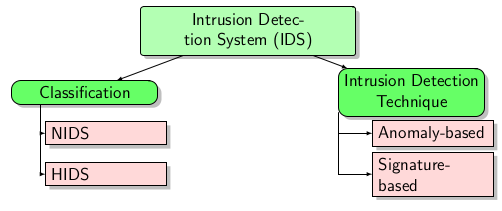
\includegraphics[width=0.8\textwidth]{Figures/IDS}
\decoRule
\caption{Fonctionnement des systèmes de détection d’intrusions}
\label{fig:IDS_Architecture}
\end{figure} 

\subsection{Les approches}
\label{approchesIDS}
Il existe deux approches d’IDS :\\
\begin{itemize}
\item[-]\textbf{Le NIDS} (Network Based IDS) assure la sécurité au niveau réseau. Il va donc écouter tout le trafic du réseau et générer des alertes en cas de comportement anormal.\\
\item[-]\textbf{Le HIDS} (Host Based IDS) réside sur une machine en particulier. Il surveille et analyse le trafic de la machine hôte pour déceler des intrusions ou des attaques (DoS par exemple). \\
\end{itemize}
Ces deux approches peuvent être fusionnées afin d’améliorer la précision de détection d’intrusion ; cette approche est appelée l’approche hybride.

\subsection{Les méthodes de détection d’intrusions} 
Il existe trois méthodes principales de détection d’intrusions:\\
\begin{itemize}
\item[•]\textbf{Détection par scénario} (Misuse Detection) : pour détecter les attaques, elle utilise une grande base de données qui contient les attaques connues et les associe aux caractéristiques des événements qui se produisent lors d’une attaque similaire. Cette technique est aussi appelée la détection basée sur la signature (Signature-Based Detection) ou la détection basée sur la connaissance (Knowledge-Based Detection).\\
\item[•]\textbf{Détection basée sur l’anomalie} (Anomaly-Based Detection) : utilise un profil qui représente les activités qui ne présentent aucune menace d’une éventuelle attaque ou une préparation d’attaque. Les événements sont par la suite comparés à ce profil d’activités.\\
\item[•]\textbf{Analyse de protocole avec état} (SPA) : commence par définir un ensemble de contraintes qui représente le comportement autorisé d’un programme ou un protocole donné. Le système surveille les opérations exécutées par le programme ou le protocole et vérifie s’ils respectent les contraintes définies par le système. 
\end{itemize} 

\subsection{Les méthodes de collection d'informations sur les flux}
Les IDS collectent les informations sur les flux en utilisant une de ces deux méthodes:\\
\begin{itemize}
\item[-] \textbf{Première méthode:} Collecter les statistiques sur les flux calculés par les switches OpenFlow.\\
\item[-] \textbf{Deuxième méthode:} Capturer les paquets avec leur renfilage et extraire les informations contenues dans ces paquets. 
\end{itemize}

\subsubsection{A) Utilisation des statistiques OpenFlow:}
La plupart des solutions de détection d’intrusions dans les SDN utilisent les statistiques calculées par les switches OpenFlow. Dans ce type de solution l’IDS est implémenté sous forme d’application SDN qui demande périodiquement les statistiques concernant les flux en utilisant le protocole OpenFlow. Les statistiques sont par la suite analysées au niveau de cette application SDN pour détecter l’intrusion. Les méthodes d’analyse sont basées sur des méthodes statistiques ou d’apprentissage automatique.

\subsubsection{B) Utilisation de l’apprentissage automatique:}
Le principe de ce type de solutions est d’utiliser un dataset (un ensemble de données) présentant des caractéristiques extraites de différents flux de paquets pour entrainer un système intelligent capable de prendre en entrée un vecteur de caractéristiques décrivant un flux de paquets et le classifier comme flux d’attaque ou flux bénins. L’efficacité de ce type de solutions est directement liée au choix du dataset, aux caractéristiques utilisées, et au modèle d’apprentissage automatique.

\subsection{Évaluation des performances d'un NIDS}
\label{evaluation}
L'efficacité du NIDS est évaluée par plusieurs paramètres. Une matrice de confusion est un tableau qui est souvent utilisé pour calculer les performances d'un NIDS. Elle est décrite dans le tableau suivant.
\begin{table}[h]
	\begin{center}
		\begin{tabular}{  | m{4cm} | m{4cm} | m{4cm} | }
			\multicolumn{3}{c}{Prédiction}\\
			\hline
			Classe réelle  & Anomalie & Légitime\\
			\hline
			Anomalie & Vrai Positif (VP) & Faux Négatif (FN)\\
			\hline
			Légitime & Faux Positif (FP) & Vrai Négatif (VN)\\
			\hline
		\end{tabular}
		\caption{Matrice de confusion}
	\end{center}
	\label{table:NIDS_Evaluation}
\end{table}

\begin{itemize}
	\item[• VP] : Le nombre d’enregistrements anomalies correctement classés.\\
	\item[• VN] : Le nombre d’enregistrements normaux correctement classés.\\
	\item[• FP] : Le nombre d’enregistrements normaux mal classés.\\
	\item[• FN] : Le nombre d’enregistrements anomalies mal classés.\\ 
\end{itemize}

Afin d'évaluer le NIDS, les métriques suivantes sont calculées :\\
\begin{itemize}
	\item[•] \textbf{Exactitude (E)}: Indique le pourcentage de prédictions correctes sur la totalité des prédictions:
	\begin{large}
		\begin{center}
			$ E = \frac{VP + VN}{ VP + VN + FP + FN} \times 100\% $
		\end{center}
	\end{large}
	
	\hfill
	
	\item[•] \textbf{Précision (P)}: Indique combien d’intrusions prédites par un NIDS sont réellement des intrusions. Plus la précision est élevée, plus le taux de fausse alerte est faible:
	\begin{large}
		\begin{center}
			$ P = \frac{VP}{ VP + FP} \times 100\%$
		\end{center}
	\end{large}
	
	\hfill
	
	\item[•] \textbf{Rappel (R)}: Pourcentage des intrusions prédites par rapport à toutes les intrusions présentées:
	\begin{large}
		\begin{center}
			$ R = \frac{VP}{ VP + FN} \times 100\%$
		\end{center}
	\end{large}
	
	\hfill
	
	\item[•] \textbf{F1-Measure (R)}: Une mesure qui combine la précision et le rappel:\\
	\begin{large}
		\begin{center}
			$ R = 2 \times \frac{1}{ \frac{1}{P} + \frac{1}{R}} \times 100\%$
		\end{center}
	\end{large}
	
	\hfill
	
	\item[•] \textbf{Taux de faux Positif (TFP) et Taux de vrai Positif (TVP)}:\\
	\begin{large}
		\begin{center}
			$ TFP = \frac{FP}{ VN + FP} \times 100\%$ , $ TVP = \frac{VP}{ VN + FP} \times 100\%$ 
		\end{center}
	\end{large}
\end{itemize}

\section{Travaux existants}
Récemment, diverses solutions ont été proposées pour régler les problèmes de sécurité au sein des réseaux SDN. Les techniques d’apprentissage automatique sont largement appliquées pour améliorer l’efficacité de détection, y compris les réseaux neurone, les arbres de décision, les SVM (Support Vector Machine) et les réseaux bayésiens. L'intégration d'un système de détection d'intrusions dans l'architecture SDN reste la meilleure solution pour sécuriser l'environnement SDN. Comme mentionné dans la section \ref{approchesIDS}, deux approches existent pour concevoir un IDS, une est basée machine (HIDS) et l'autre est basée réseau (NIDS), autrement appelé basé flux. Dans notre travail nous nous focaliserons sur les systèmes de détection basés flux, donc nous allons présenter en ce qui suit quelques IDS déjà existants afin de pouvoir faire une étude comparative; technique d'apprentissage adoptée, les caractéristiques utilisées, le dataset, résultat de prédiction.\\

\newpage
\subsection{Flow based Intrusion Detection System [\cite{11}]:}
Les auteurs de ce travail ont proposé un système de détection basé flux pour détecter le trafic anormal circulant dans les réseaux SDN. Leur IDS est basé sur l’extraction d’un ensemble de caractéristiques prédéfinies de manière régulière chaque une seconde. Cette étape est suivie par l’agrégation des caractéristiques extraites pour pouvoir traîner le modèle. La figure \ref{fig:NIDS1} illustre l'architecture de cette IDS.
\begin{figure}[h]
\centering
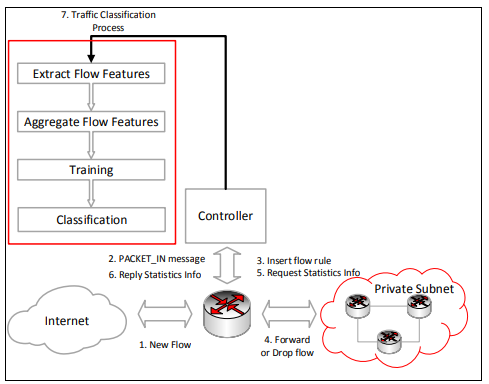
\includegraphics[width=0.6\textwidth]{Figures/NIDS1}
\decoRule
\caption{IDS [\cite{11}]}
\label{fig:NIDS1}
\end{figure}

\subsubsection{A) Extraction et agrégation des caractéristiques:}
Les commutateurs OF envoient souvent des messages \textit{Packet-In} au contrôleur quand aucune correspondance n’est trouvée dans la table de flux du commutateur. Chaque message contient les informations du premier paquet de chaque flux et quand il est reçu au niveau du contrôleur ces informations sont extraites et sauvegardées. En plus, ce qui est bien avec les SDN, ces commutateurs peuvent envoyer des statistiques pour chaque entrée de flux, ce qui permettra la collecte d'informations de flux chaque seconde. 

\subsubsection{B) Entraînement do modèle et la classification:}
Les échantillons extraits de la phase d’agrégation sont utilisés dans un modèle de classification supervisé. Par conséquent, le classificateur formé attribuera des classes à chaque échantillon chaque seconde. Puisque chaque flux peut avoir plus d’une instance au cours de sa durée de vie, son comportement sera classé plusieurs fois. Le classifieur \textit{Bagged-Trees} [\cite{12}] a été utilisé pour construire le modèle.
\newpage
\subsection{Machine based Intrusion Detection System [\cite{13}]:}
Dans ce travail un modèle de réseaux de neurones a été intégré dans le système pour détecter les anomalies dans le trafic. Le système fonctionne comme suit; les commutateurs OF envoient périodiquement les statistiques de flux au contrôleur, ces statistiques vont être récupérées et traitées par le module responsable pour détecter le comportement d’anomalie dans le flux. Pattern recognition (la reconnaissance de motifs) est implémentée dans ce modèle pour classer les entrées dans un ensemble de catégories cibles. L’architecture de cet IDS se compose de trois couches : une couche d’entrée (Input Layer), une couche cachée (Hidden Layer) et une couche de sortie (Output Layer). L’algorithme "\textbf{Backpropagation}" est utilisé pour traîner le modèle.\\

\begin{table}[h]
\begin{center}
\begin{tabular}{  | m{4cm} | m{5cm} | m{5cm} | }
\hline
IDS & Machine based Intrusion Detection System [\cite{13}] & Flow based Intrusion Detection System [\cite{11}]\\
\hline
Technique d’apprentissage automatique & Neural Network & Bagged Trees\\
\hline
Caractéristiques utilisées & \begin{itemize}
\item[-] Durée
\item[-] Type de protocole
\item[-] Nombre d’octets source-destination
\item[-] Nombre d’octets destination-source
\item[-] Nombre de connections avec le même hôte
\item[-] Nombre de connections vers le même service
\end{itemize} &\begin{itemize}
\item[-] Durée de mesure
\item[-] Nombre de paquets
\item[-] Nombre d’octets
\item[-] Variation dans la durée du flux
\item[-] Variation dans le nombre de paquets
\item[-] Variation dans le nombre d’octets
\end{itemize} \\
\hline
Dataset & NSL-KDD (standardisé) crée en 1999 & Généré avec une émulation de l’environnement SDN (non standardisé) publiée en 2017 \\
\hline 
Type d’attaques dans le dataset  & \begin{itemize}
\item[-] DoS
\item[-] Remote2Local
\item[-] User2Root
\item[-] Probe
\end{itemize} &\begin{itemize}
\item[-] DoS
\item[-] Http brute force
\item[-] SSH brute force
\end{itemize}\\
\hline
\end{tabular}
\caption{Comparaison entre les deux IDS proposés}
\end{center}
\label{table:IDS}
\end{table}

\begin{tabular}{| m{4cm} | m{5cm} | m{5cm} |}
\multicolumn{3}{c}{Résultats expérimentaux}\\
\hline
Taux de vrai Positif & 0.941 & 0.9834\\
\hline
Taux de faux Positif & 0.005 & 0.016\\
\hline
Exactitude & 0.973 & Non mentionnée \\
\hline
\end{tabular}

\subsection{Comparaison entre ces deux IDS}
Nous remarquons que les deux solutions donnent des résultats de performances très intéressants. Les auteurs de la solution [\cite{11}] n’ont pas mentionné le taux de faux négatifs qu’est un élément très important dans l’évaluation d’un IDS. L’utilisation d’un dataset non standardisé dans [\cite{11}] est discutable sur le plan de la validité des attaques, les flux générés et le bon déroulement de l’extraction des informations et caractéristiques lors de la création du dataset. La solution [\cite{13}] utilise un ancien dataset(NSL-KDD créé en 1999) qui s’avère dépassé dû aux grands changements dans les réseaux, et l’apparition de nouveaux types d’attaques récentes. Par conséquent, l’IDS peut être inefficaces face aux attaques récentes ainsi que dans la reconnaissance des caractéristiques des flux normaux modernes.\\
D’après cette étude nous constatons qu’il est nécessaire de mettre en place une solution de détection des attaques DoS dans les SDN qui prend en considération les critiques susmentionnées. 

\section{Conclusion}
Dans ce chapitre nous avons tout d’abord étudié les problèmes de sécurité dans l’environnement SDN. Nous avons ensuite présenté quelques solutions déjà proposées pour détecter les attaques Dos. Dans le chapitre suivant, nous allons nous familiariser avec la technique d’apprentissage que nous utiliserons pour la conception de nore solution. 